%================================================================
%                           N O T E S
%                           ---------
%
%                           ---------
%-----------------------------------------------------------------
%                       INTRODUCTION
%-----------------------------------------------------------------
\section{Introduction}
%
The goal of this tool was to plot the scattered field. I took Prof. Guettel's Introduction to Python in 2nd Year and was interested in learning more about using the language. \par
%
I started off with a text file on my laptop but quickly realised I would benefit from version controlling it, so I created a repository on Bitbucket. You can access it \href{https://bitbucket.org/veracruz/canonical_scattering}{here}. It also helped me version control this document, since it became quite complex quickly. \par
%
In Prof. Guettel's introduction to Python we exclusively used functions to build a game of Othello that ran in the command line. This is very different to what I have done here, where I would need the programme to output the file of the plotted field. Additionally, this tool became many orders of magnitude more complex because of the nature of the problem and I thought it appropriate to employ an object oriented approach.\par
%
TODO: I need to credit Nathan but I'm not sure how to go about it.\par
%
I used four different libraries for this project, namely \verb!numpy!, \verb!matplotlib.pyplot!, \verb!scipy.special! and \verb!mpmath!.
%
%-----------------------------------------------------------------
%                       THE SET UP
%-----------------------------------------------------------------
\section{Approach}
%
My tool is set up in two files: \verb!plotter.py! and \verb!fields.py!. These can be found in the Bitbucket repository above. \par
%
The \verb!plotter.py! file holds three classes: \verb!Main!, \verb!Wave! and \verb!Graphics!. The \verb!fields.py! file holds subclasses which are instantiations of the \verb!Wave! class, the most important of which is \verb!CylinderField(Wave)!, which provides the fields calculated in Chapter 2.\par
%
Within the \verb!Main! class I defined the \verb!run! class, which runs the tool when it is compiled as a python script from the command line. I also define different functions for different fields I want to plot in this class, so that it is easy to call them. For example, for the cylinder scattering problem I call
%
  \begin{lstlisting}
self.create_field_around_cylinder(self.graph) \end{lstlisting}
%
where I have defined
%
  \begin{lstlisting}
def create_field_around_cylinder(self, graph):
    field = CylinderField()
    graph.heat_map(field) \end{lstlisting}
%
and \verb!self.graph = Graphics! was set within the \verb!__init__! constructor method.
%
%-----------------------------------------------------------------
%                      Graphics class
%-----------------------------------------------------------------
\section{The \texttt{Graphics} class}
%
The \verb!Graphics! class is equipped with two different types of plots: \verb!heat_map! and \verb!contour!. Both of these are constructed in the same way:
%
  \begin{lstlisting}[caption={},label={lst:contour}]
def contour(self, wave, xlabel='x', ylabel='y'):
    plt.contour(wave.get_Z(), extent=wave.get_extent())
    self.label_plot(wave, xlabel, ylabel)
    self.draw_plot() \end{lstlisting}
%
where \verb!contour! is replaced by \verb!imshow! for the heat map. \par
%
Here the specific wave instantiation, \verb!wave!, is fed through to the \verb!contour! function in \verb!matplotlib.pyplot! which returns the set of contour lines for the heights given by \verb!wave.get_Z!. I then add labels to my plot, and the \verb!draw_plot! function draws it. \par
%
The \verb!label_plot! function looks for the title I have set for my wave instantiation using the \verb!wave.get_name! function, along with labels for the axes. \par
%
The plotting function brings it all together
%
  \begin{lstlisting}
def draw_plot(self, wave):
    self.draw_disk_overlay(wave)
    plt.colorbar()
    plt.show()\end{lstlisting}
%
where the \verb!draw_disk_overlay! function creates a solid disk in the plot to block out the area where the field should not be calculated inside the cylinder. The size of this disk is pulled from the specific wave instantiation using \verb!get_cylinder_radius! and plotted with \verb!pyplot!.
%
\begin{lstlisting}
def draw_disk_overlay(self, wave):
    r = wave.get_cylinder_radius()
    plt.gca().add_patch(plt.Circle((0,0),r, fc='#36859F'))
\end{lstlisting}
%
%-----------------------------------------------------------------
%                      Wave() class
%-----------------------------------------------------------------
\section{The \texttt{Wave} class}
%
This is fairly big class but its functions can be divided up into three main categories: plot information, constants, and mathematical functions. It makes sense to keep them all within one class because all the specific wave instantiations will make use of these functions. \par
%
%------------------ plot information --------------------------------
\subsection{Plot information}
Throughout this project I have attempted to name my functions to best represent the action they perform. For instance \verb!get_wavevector! returns the wavevector, \verb!self.wavevector!, whereas \verb!set_wavevector(k)! sets \verb!k! \verb!=! \verb!self.! \verb!wavevector!. This is especially useful when setting and retrieving these constants within the specific wave instantiations. \par
%
Following this convention I have a series of functions that set or retrieve information about the specific plot. \par
%
The functions \verb!set/get_name,! set and retrieve the name of the plot; \verb!get_X,! \verb!get_Y! and \verb!get_Z! retrieve the three coordinate arrays; \verb!set/get_! \verb!axis_! \verb!length! and set and retrieve the range of \verb!x! and \verb!y!; \verb!set/get_! \verb!axis! \verb!_delta! set and retrieve the granularity of the plot. \par
%
The axis length functions are additionally also used to specify an `extent' function, \verb!get_extent!, which is used in the \verb!Graphics! class to make sure the axis labels in the plot are over the correct range (see \ref{lst:contour}). \par
%
  \begin{lstlisting}
def get_extent(self):
    return [-self.get_axis_length(), self.get_axis_length(),
        -self.get_axis_length(), self.get_axis_length()] \end{lstlisting}
%
Finally, the \verb!Wave! class is initalised by setting the arrays that will constitute our domain: \verb!self.X, self.Y = self.get_xy_series()!, where this function is defined as follows.
%
  \begin{lstlisting}
def get_xy_series(self):
    x = np.linspace(-self.get_axis_length(),
        self.get_axis_length(), self.get_axis_delta())
    y = x
    return np.meshgrid(x, y)\end{lstlisting}
%
TODO: need to fix how x and y are defined.\par
%
Now that we have defined the cartesian coordinates $x$ and $y$, we can use them to define $r$ and $\theta$. We define $r$ as follows, using the \verb!numpy! library:
%
  \begin{lstlisting}
def get_r(self):
    return np.sqrt( self.get_X()*self.get_X()
        + self.get_Y()*self.get_Y() )\end{lstlisting}
%
TODO: explain why $x*x$ instead of $x^2$.\par
%
The angular coordinate is particularly interesting because it needs work in all four quadrants of our plotted field. \verb!Numpy! offers two versions of the $\arctan(\theta)$ function, \verb!numpy.arctan! and \verb!numpy.! \verb!arctan2!. The first returns the angle $\theta \in [\frac{\pi}{2},\frac{\pi}{2}]$, that is, $(x, y)$ in the rightmost quadrants. We don't expect our field to be symmetric around $x=0$, so we need to use the latter function, which returns $\theta \in [\pi, -\pi]$.
%
  \begin{lstlisting}
def get_theta(self):
    return np.arctan2(self.get_X(), self.get_Y())\end{lstlisting}\par
%
%--------------------- wave constants -----------------------------
\subsection{Wave constants}
%
The second set of functions defined within the \verb!Wave! class consist of the physical constants of the problem. These are determined by the wavenumber, which is set and retrieved using \verb!get/set_wavevector! for each wave instantiation. The wavevector is an array length two, such that $\vec{k} = (a,b) = (kcos\alpha, ksin\alpha)$.\par
%
From this wave vector we can calculate the wavenumber, $k$,
%
  \begin{lstlisting}
def get_wavenumber(self):
    return np.sqrt(self.wavevector[0]*self.wavevector[0]
        + self.wavevector[1]*self.wavevector[1])\end{lstlisting}
%
the incident angle, $\alpha$, again using \verb!arctan2!:
%
  \begin{lstlisting}
def get_incident_angle(self):
    return np.arctan2(self.wavevector[0], self.wavevector[1])\end{lstlisting}\par
%
For the purposes of this project, I set the speed of sound to 343 $ms^{-1}$. Now we can calculate $\omega = k c$, the frequency of the wave (see Definition \ref{defn:frequency}).
%
  \begin{lstlisting}
def get_omega(self):
    return self.get_speed_of_sound()*self.get_wavenumber()\end{lstlisting} \par
%
Our solution deals with sums to infinity, so we must set a truncation numer. This is done with \verb!get/set_truncation!. Similarly, we need to specify the radius of the circle we are concerned with. This is set and retrieved using \verb!get/set_cylinder_radius!.
%
%--------------------- math functions -----------------------------
\subsection{Mathematical functions}
%
Finally, we describe the Neumann factor, as defined in \ref{propn:jacobi_expansion}. I added an error message to make sure the function behaves as expected.
  \begin{lstlisting}
def get_neumann_factor(self, n):
      if n==0:
          return 1
      elif n > 0:
          return 2
      else:
          print('ERROR: Invalid n for Neumann factor')\end{lstlisting}
%
\section{Particular \texttt{Wave} instantiations}
%
All the classes in this file are subclasses of \verb!Wave!. They are initialised with the superconstructor referring back to the parent class so that they all inherit the functions and variables of \verb!Wave()!.
%
  \begin{lstlisting}
def __init__(self):
    print('[Field_name] started...')

    self.set_parameters()
    self.set_name("Example name")

    super(Field_name, self).__init__()

    self.Z = self.get_z_series()\end{lstlisting}\par
%
Note that the superconstructor needs to go stricly \textit{after} the parameters are set. This is to override any defaults I have set in \verb!Wave!. The \verb!set_paramaters! function sets the specific values for the wavevector, truncation number, radius, and the range and granularity of the grid. \par
%
The array \verb!self.Z! is what \verb!Graphics! will plot. Each value in this array will be calculated by a (truncated) infinite sum depending on the coordinates $r$ and $\theta$.
%
  \begin{lstlisting}
def get_z_series(self):
    return self.get_sum(self.get_r(), self.get_theta()) \end{lstlisting}
%
We can now exploit the fact that our solutions for this field are separable to write
  \begin{equation}
    \text{total field} = \text{constant terms} \cdot \text{angular terms} \cdot \text{radial terms}.
  \end{equation}\par
%
  \begin{lstlisting}
def get_sum(self, r, theta):
    z = 0       #Initialising
    for n in range(self.truncation):
        z += self.get_constant_term(n) * self.get_angular_term(n, theta) * self.get_radial_term(n, r)
    return z.real   \end{lstlisting}\par
%
We can now define what these constant, angular and radial terms are for each specific field.
%
%--------------------------- cylinder -------------------------------
\subsection{The scattered field around a cylinder}
%
\subsubsection{Constant term}
In this case, we have two types of constant terms: Neumann or Dirichlet. One could choose to define two separate functions \verb!get_dirichlet_constants! and \verb!get_neumann_constants!, but I've simply defined my function to take a \verb!type! argument which is set to Neumann by default. I added an error message to make sure the function behaves as expected.
%
  \begin{lstlisting}
def get_constant_term(self, n, type='neumann'):
    if type == 'neumann':
        return self.get_neumann_factor(n) * np.power(1j,n) * self.get_neumann_bc(n)
    elif type == 'dirichlet':
        return self.get_neumann_factor(n) * np.power(1j,n) * self.get_dirichlet_bc(n)
    else:
        print('ERROR: Invalid type in CylinderField.get_constant_term') \end{lstlisting} \par
%
Where \verb!get_neumann_bc! and \verb!get_dirichlet_bc! are defined as follows.
%
  \begin{lstlisting}
def get_neumann_bc(self, n):
    return sp.jvp(n, self.get_wavenumber() * self.get_cylinder_radius()) / sp.h1vp(n, self.get_wavenumber() * self.get_cylinder_radius()) \end{lstlisting} \par
%
  \begin{lstlisting}
def get_dirichlet_bc(self, n):
    return None #TBD \end{lstlisting}\par
%
The function \verb!sp.jvp(v, z, m=1)! computes the $m^{th}$ derivative of the Bessel function of the first kind of order $v$ and argument $z$. It is provided by the \verb!scipy.special! library, imported as \verb!sp! here. Similarly \verb!sp.h1vp(v, z, m=1)! computes the $m^{th}$ derivative of the Hankel function of the first kind of order $v$ and argument $z$.

\subsubsection{Radial dependence}
%
  \begin{lstlisting}
def get_radial_term(self, n, r):
    return ( sp.hankel1(n, self.get_wavenumber() * r) + sp.jv(n, self.get_wavenumber() * r))\end{lstlisting}
%
\subsubsection{Angular dependence}
%
  \begin{lstlisting}
def get_angular_term(self, n, theta):
    return np.cos(n * (theta - self.get_incident_angle()))\end{lstlisting}
%
\section{Secondary plots}\label{ss:secondary_plots}
I used python to create most of the figures in this document.
%
  \begin{lstlisting}[caption={Plot of bessel functions of integer order},label={lst:bessel_int_no}]
x=np.linspace(0,5,100)

fig=plt.figure()
ax=fig.add_subplot(111)

for n in range(6):
    ax.plot(x,sp.jv(n, x), label=str(n))

plt.axhline(color='black',
            linewidth = 0.5)

plt.legend(loc=1)
plt.title('Bessel function of order n.')
plt.show()\end{lstlisting}\par
%
The code for the Neumann functions plot was similar, replacing \verb!sp.jv(n,x)! on line 7 by \verb!sp.yn(n,x)!. I also had to adjust the axis to make sure we got a meaningful plot, see \figref{fig:neumann_bounding_axis}.\par
%
\begin{figure} \centering
  %
  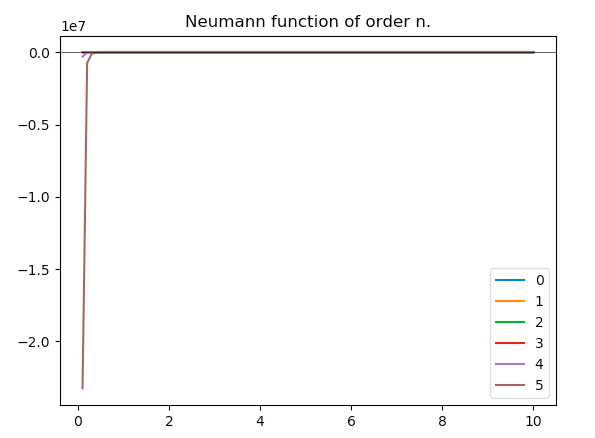
\includegraphics[width=6cm]{../figures/plot_neumann_unbounded_y}
  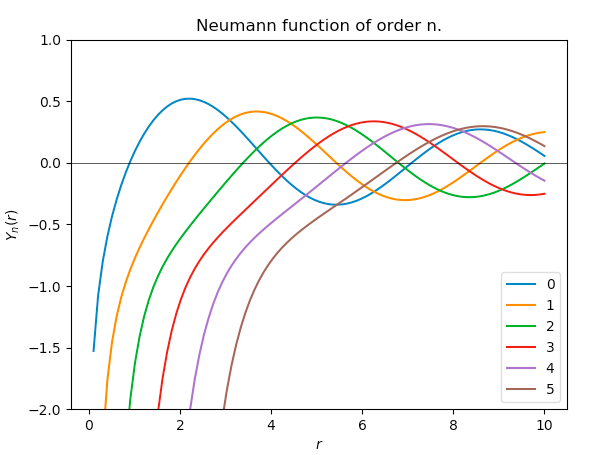
\includegraphics[width=6cm]{../figures/plot_neumann_int_order}
  \caption{Neumann functions with and without bounded axis}\label{fig:neumann_bounding_axis}
  %
\end{figure}
%
\begin{lstlisting}[caption={Plot of neumann functions of integer order},label={lst:neumann_int_no}]
x=np.linspace(0,10,100)

fig=plt.figure()
ax=fig.add_subplot(111)

axes = plt.gca()
axes.set_ylim([-2,1])

for n in range(6):
    ax.plot(x,sp.yn(n, x), label=str(n))

plt.axhline(color='black',
            linewidth = 0.5)

plt.legend(loc=4)
plt.title('Neumann function of order n.')
plt.show()\end{lstlisting}\par
%
For Hankel functions I decided to plot the absolute value. If we do not specify when plotting, \verb!matplotlib! takes the real part of a complex number, so withou the \verb!abs! command this was just plotting a Bessel function.
%
\begin{lstlisting}[caption={Plot of hankel functions of integer order},label={lst:hankel_int_no}]
x=np.linspace(0,7,100)

fig=plt.figure()
ax=fig.add_subplot(111)

axes = plt.gca()
axes.set_ylim([0,4])

for n in range(6):
    ax.plot(x,abs(sp.hankel1(n, x)), label=str(n))

plt.legend(loc=1)
plt.title('Absolute value of the Hankel function of the first type of order n.')
plt.ylabel('$H_{n}^{(1)}(r)$')
plt.xlabel('$r$')
plt.show()\end{lstlisting}\par
